\pdfoutput=1
\documentclass[a4paper,pdflatex,ja=standard]{bxjsarticle}

% ---Display \subsubsection at the Index
% \setcounter{tocdepth}{3}

% ---Setting about the geometry of the document----
% \usepackage{a4wide}
% \pagestyle{empty}

% ---Physics and Math Packages---
\usepackage{amssymb,amsfonts,amsthm,mathtools}
\usepackage{physics,braket,bm}

% ---underline---
\usepackage{ulem}

% ---cancel---
\usepackage{cancel}

% --- surround the texts or equations
% \usepackage{fancybox,ascmac,tcolorbox}

% ---settings of theorem environment---
% \usepackage{amsthm}
% \theoremstyle{definition}

% ---settings of proof environment---
% \renewcommand{\proofname}{\textbf{証明}}
% \renewcommand{\qedsymbol}{$\blacksquare$}

% ---Ignore the Warnings---
\usepackage{silence}
\WarningFilter{latexfont}{Some font shapes,Font shape}

% ---Insert the figure (If insert the `draft' at the option, the process becomes faster.)---
% \usepackage{graphicx}
% \usepackage{subcaption}

% ----Add a link to a text---
\usepackage{url}
\usepackage{xcolor,hyperref}
\hypersetup{colorlinks=true,citecolor=orange,linkcolor=blue,urlcolor=magenta}
\usepackage[whole,autotilde]{bxcjkjatype}

% ---Tikz---
% \usepackage{tikz,pgf,pgfplots,circuitikz}
% \pgfplotsset{compat=1.15}
% \usetikzlibrary{intersections,arrows.meta,angles,calc,3d,decorations.pathmorphing}

% ---Add the section number to the equation, figure, and table number---
\makeatletter
   \renewcommand{\theequation}{\thesection.\arabic{equation}}
   \@addtoreset{equation}{section}
   
   \renewcommand{\thefigure}{\thesection.\arabic{figure}}
   \@addtoreset{figure}{section}
   
   \renewcommand{\thetable}{\thesection.\arabic{table}}
   \@addtoreset{table}{section}
\makeatother

% ---enumerate---
% \renewcommand{\labelenumi}{$\arabic{enumi}.$}
% \renewcommand{\labelenumii}{$(\arabic{enumii})$}

% ---Index---
% \usepackage{makeidx}
% \makeindex 

% ---Fonts---
% \renewcommand{\familydefault}{\sfdefault}

% ---Title---
\title{高校物理で分かるかもしれないアハラノフ・ボーム効果}
\author{ミヤ}
\date{最終更新:\today}

\begin{document}

\maketitle

\tableofcontents

\clearpage
\section{はじめに}

本稿では,高校物理で習う電磁波の回折・干渉の実験のみを基礎知識として,量子力学との関連を調べていく.これらの理論は,電磁気学の共変形式,すなわち相対性理論との関係が深く,それらは高校物理から少し逸脱するため,ここでは関係する知識をはじめに確認することにする.

後半では,アハラノフ・ボーム効果について,筆者が調べたことをまとめているが,そもそもこういった議論は様々な思想が入り混じっており\textbf{真に受けると色々と大変}なので,エンタメとして楽しんでいただければと思っている.


\section{ゲージ場と量子力学}

アハラノフ・ボーム効果は,量子力学の枠組みで電磁気学を語ろうとするときに表れる現象である.これから解説する通り,アハラノフ・ボーム効果は古典論的な直感に反する現象である.その効果は実験的にも実証されており\footnote{
  アハラノフ・ボーム効果の検証は日本人のグループによって精力的に研究されていた.この実験的な検証はノーベル賞級と言われていたが,その業績の筆頭である外村先生は2012年に亡くなられてしまった(ちなみに,外村先生の論文\cite{Tonomura_ObservationAharonovBohm_1982}がJ.J.サクライの教科書\cite{J.J.Sakurai_ModernQuantum_1985}で引用されていた.ちょっとうれしかった.).
},量子力学の有効性を示している1つの根拠になりうるだろう.

\subsection{古典論における電磁気学とゲージ場の関係}

古典的な電磁場$\bm{E}(\bm{x},t),\bm{B}(\bm{x},t)$の振る舞いは,マクスウェル方程式といわれる4つの方程式
\begin{equation}
  \left\{
    \begin{alignedat}{1}
      \bm{\nabla}\cdot\bm{E}
      &=
      \rho
      \\
      \bm{\nabla}\cdot\bm{B}
      &=
      0
      \\
      \bm{\nabla}\times\bm{E}+\pdv{\bm{B}}{t}
      &=
      \bm{0}
      \\
      \bm{\nabla}\times\bm{B}
      -
      \pdv{\bm{E}}{t}
      &=
      \bm{j}
    \end{alignedat}
  \right.
  \label{maxwell_eq}
\end{equation}
によって決定される\footnote{
  本稿では$c=\hbar=1$に加えて,$\varepsilon_0=\mu_0=1$とする.
}.もちろん,マクスウェル方程式はこのままでも良いのだが,この表式ではいくつかの疑問が生じる.それらは例えば,方程式として解くべき関数の数が6つ(電場と磁場がそれぞれ3成分)あるのに対して方程式が8つもあったり,ローレンツ不変性が明らかではないということである.

これらの疑問はかなり本質的であり,もちろん答えがあるが,いったんそれらを先送りにしてマクスウェル方程式をもう少し書き換えてみよう.実は第2式と第3式に注目すると,解の形が決まってくることが分かってくる.ここでは,電磁場$\bm{E}(\bm{x},t),\bm{B}(\bm{x},t)$を新しい場$\phi(\bm{x},t),\bm{A}(\bm{x},t)$を用いて
\begin{equation}
  \bm{E}(\bm{x},t)
  =
  -
  \bm{\nabla}\phi
  -
  \pdv{\bm{A}}{t}
  ,\quad 
  \bm{B}(\bm{x},t)
  =
  \bm{\nabla}\times\bm{A}
  \label{gauge_elemag}
\end{equation}
と書いてみよう\footnote{
  少し先走った脚注であるが,このように書いた場合,ローレンツの添え字には気をつけなくてはならない.ここでは,ベクトルポテンシャルは反変ベクトルだとして,ローレンツの添え字$\mu$は上に書いたものと対応させることにする.つまり,$A^{\mu}=(\phi,\bm{A})$である.
  \label{note3}
}.すると,これらは確かにマクスウェル方程式の第2式と第3式を満たしている.実際,ベクトル解析の公式を用いれば
\begin{gather}
  \bm{\nabla}
  \cdot
  \bm{B}
  =
  \bm{\nabla}
  \cdot
  (\bm{\nabla}\times\bm{A})
  =
  0
  \\
  \bm{\nabla}
  \times
  \bm{E}
  +
  \pdv{\bm{B}}{t}
  =
  -
  \bm{\nabla}\times(\bm{\nabla}\phi)
  -
  \pdv{}{t}
  (\bm{\nabla}\times\bm{A})
  +
  \pdv{}{t}
  (\bm{\nabla}\times\bm{A})
  =
  \bm{0}
\end{gather}
となっている.

では,マクスウェル方程式\eqref{maxwell_eq}の残りは,ここで定義したゲージ場$\phi,\bm{A}$を用いてどのように書けるだろうか?この書き換えを行うためには,次の電磁場テンソルと4元電流密度ベクトル
\begin{equation}
  F^{\mu\nu}
  =
  \partial^{\mu}A^{\nu}
  -
  \partial^{\nu}A^{\mu}
  ,\ 
  j^{\mu}
  =
  (\rho,\bm{j})
  \label{elemag_tensor}
\end{equation}
を定義しておくと見通しが良い.ここで,$A^{\mu}=(\phi,\bm{A})$である\footnote{
  慣れない人にはこの書き方は不親切かもしれない.ある4元ベクトル$V^{\mu}$に対して,$V^{\mu}=(V_{\phi},\bm{V})$のように書いた場合は
  $$
    V^{0}=V_{\phi}
    ,\ 
    V^{1}=V_x
    ,\ 
    V^{2}=V_y
    ,\ 
    V^{3}=V_z
  $$
  と定義する.
  \label{note4}
}.この様に定義しておけば,マクスウェル方程式\eqref{maxwell_eq}の第1式と第4式は
\begin{equation}
  \partial_{\mu}F^{\mu\nu}
  =
  j^{\nu}
  \quad
  (\nu=0,1,2,3)
  \label{maxwell_covariant}
\end{equation}
に対応する.このことを確認するためには
\begin{equation}
  F^{\mu\nu}
  =
  \begin{pmatrix}
    F^{00} & F^{01} & F^{02} & F^{03}  \\
    F^{10} & F^{11} & F^{12} & F^{13}  \\
    F^{20} & F^{21} & F^{22} & F^{23}  \\
    F^{30} & F^{31} & F^{32} & F^{33} 
  \end{pmatrix}
  =
  \begin{pmatrix}
    0 & -E_x & -E_y & -E_z \\
    E_{x} & 0 & -B_z & B_y \\
    E_{y} & B_z & 0 & -B_x \\
    E_{z} & -B_y & B_x & 0
  \end{pmatrix}
\end{equation}
となっていることを示して\footnote{
  電磁場テンソルの符号には注意する必要がある.ここでは,脚注\ref{note4}のように定義しているので,例えば
  $$
    F^{01}
    =
    \partial^{0}A^{1}
    -
    \partial^{1}A^{0}
    =
    -
    \left(  
      -
      \pdv{\phi}{x}
      -
      \pdv{A_x}{t}
    \right)
    =
    -E_x
  $$
  である.他の定義(例えばWikipedia)とは違うので注意.
},
\begin{align}
  &
  \partial_{\mu}F^{\mu 0}=j^{0}
  \ 
  \rightarrow
  \ 
  \bm{\nabla}
  \cdot
  \bm{E}
  =
  \rho
  \\
  &
  \partial_{\mu}F^{\mu i}=j^{i}
  \ 
  \rightarrow
  \ 
  \bm{\nabla}\times\bm{B}
  -
  \pdv{\bm{E}}{t}
  =
  \bm{j}
\end{align}
になることを確かめればいい.

以上の議論をまとめると,マクスウェル方程式
\begin{equation}
  \left\{
    \begin{alignedat}{1}
      \bm{\nabla}\cdot\bm{E}
      &=
      \rho
      \\
      \bm{\nabla}\cdot\bm{B}
      &=
      0
      \\
      \bm{\nabla}\times\bm{E}+\pdv{\bm{B}}{t}
      &=
      \bm{0}
      \\
      \bm{\nabla}\times\bm{B}
      -
      \pdv{\bm{E}}{t}
      &=
      \bm{j}
    \end{alignedat}
  \right.
  \tag{\ref{maxwell_eq}}
\end{equation}
は,電磁場テンソルと電流密度ベクトル\eqref{elemag_tensor}を用いれば
\begin{equation}
  \partial_{\mu}F^{\mu\nu}
  =
  j^{\nu}
  \quad
  (\nu=0,1,2,3)
  \tag{\ref{maxwell_covariant}}
\end{equation}
と等価である.元々の方程式\eqref{maxwell_eq}の第2式と第3式は,ベクトル場$A^{\mu}=(\phi,\bm{A})$をセッティングした時点で成立しているので,\eqref{maxwell_covariant}のみをマクスウェル方程式と呼ぶことが多い\footnote{
  元々のマクスウェル方程式\eqref{maxwell_eq}の第2式と第3式は,このような事情から「自明な関係式」と呼ぶことが多い.これらは,共変形式では\textbf{ビアンキ恒等式}
  $$
    \varepsilon^{\mu\nu\rho\sigma}
    \partial_{\nu}F_{\rho\sigma}
    =
    0
    \quad
    (\mu=0,1,2,3)
  $$
  に対応する.
}.さて,これで,先送りにしていた2つの疑問に答えることができる.それらは「式の自由度」と「ローレンツ不変性」であった.式の自由度については,未知の場が$\phi,A_x,A_y,A_z$と4つなのに対し,それらを決定する式は\eqref{maxwell_covariant}と4つになっており,ちゃんと未知の関数と拘束条件の数が一致している.ローレンツ不変性に対しては明らかだろう.

\vspace{10pt}
{\small
  ちなみに,共変形式を考えなくてもこれらの疑問には答えることができる.方程式の自由度については,時間変化を含まない方程式は,実質的に時間発展には効いてこない(それらは初期条件に効いてくる)ので,方程式は実は6つだし,ローレンツ不変性も電磁場のローレンツ変換を考えれば一応は確かめることができる.
}


\subsection{ゲージ不変性}

さて,共変形式でマクスウェル方程式が書けたが,そこから読み取れる事実として\textbf{ゲージ不変性}があるのでそれを確認しよう.

ゲージ不変性の概念自体は簡単である.電磁場テンソル$F^{\mu\nu}$はゲージ場を用いた定義\eqref{elemag_tensor}から
\begin{equation}
  \tilde{A}_{\mu}(x)
  =
  A_{\mu}(x)
  -
  \partial_{\mu}\alpha(x)
\end{equation}
という変換に対して変わらないことが分かる.ここで,$\alpha(x)$はスカラーの関数である.この変換を\textbf{ゲージ変換}という.この変換に対して不変であるということは,例えば,変換後の電磁場テンソルを$\tilde{F}^{\mu\nu}$とすれば,
\begin{align}
  \tilde{F}^{\mu\nu}
  &=
  \partial^{\mu}\tilde{A}^{\nu}
  -
  \partial^{\nu}\tilde{A}^{\mu}
  \nonumber
  \\
  &=
  \partial^{\mu}(A^{\nu}-\partial^{\nu}\alpha)
  -
  \partial^{\nu}(A^{\mu}-\partial^{\mu}\alpha)
  \nonumber
  \\
  &=
  \partial^{\mu}A^{\nu}
  -
  \partial^{\nu}A^{\mu}
  =
  F^{\mu\nu}
\end{align}
となることから分かる.このことから,電磁場もゲージ変換に関して不変なことが分かる.

したがって,今ここで話している古典論の世界は,ゲージ変換に対して全く物理法則が変わらないことを示している.このことを\textbf{対称性}というが,物理学では一般に\textbf{対称性のある量は観測することができない}という原則がある.ここでいう「対称性のある量」というのは,不変量という意味ではなく,対称性により生じる自由度のある量という意味で用いている.例えば「宇宙は等方一様である」といった場合は宇宙の絶対的な方角みたいなものは観測できないが,距離などは測定できる.また,「時間対称」と言われたら基本的には絶対的な時間の向きは分からない.ゲージ場についても同様で,もしこの世界の物理法則がゲージ不変なら,ゲージ不変な量は測定できるがゲージ場$A^{\mu}$という量は観測できないのである.

\vspace{10pt}
{\small
  こういった議論は少し注意が必要である.例えば,理論が時間対称であっても時間の流れは過去から未来へと一方向へ進んでいるように思えるし,理論がローレンツ対称といっても色々なローレンツ不変な観測量が測定できてしまうように思える.こういった対称性にまつわる議論は場の量子論,特にその現象論的な観点からみると面白いが,ここでは「対称性のある量は観測できない」と割り切っておこう.
}
\vspace{10pt}

以上から,(古典論で考えている限りは)ゲージ場$A^{\mu}$はマクスウェル方程式を見やすくするためのツールに過ぎないという解釈ができる.その立場に立つと,私たちが実際に観測できるのは電磁場$\bm{E},\bm{B}$であり,ゲージ場を用いても用いなくても良いのである.

\subsection{量子力学におけるゲージ場}

これまでの文章で「古典論で議論している限りは」といったような文言が散見されていたことから予想できると思われるが,理論を量子論に移行すると,少し事情が変わってくる.その例が\textbf{アハラノフ・ボーム効果}である.

アハラノフ・ボーム効果は,二重スリット実験を例にとって考えると分かりやすいだろう.二重スリット実験では,粒子の波動関数が移動する経路の長さに応じて位相が変化することから,波の干渉実験と同じような干渉縞が出現するという実験であった.ここでは,さらにある一定領域のみに磁場を発生させた場合を考えよう(図\ref{two_slit}).このとき,干渉縞は変わるのだろうか,というのが私たちがこれから考える問いである.

\begin{figure}[ht]
  \centering
  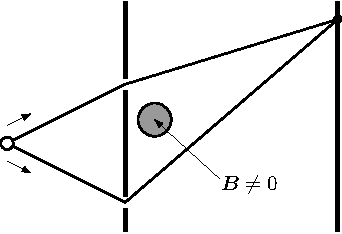
\includegraphics{fig/two_slit.pdf}
  \caption{二重スリット実験に磁場を追加する(灰色の部分に磁場がある)}
  \label{two_slit}
\end{figure}

ひとまず,量子論でこの状況を定式化してみることにしよう.ある程度,量子力学が分かっている人から見れば,経路積分による定式化をすれば素直である.例えば,自由粒子のラグランジアンは
\begin{equation}
  L_0
  =
  \frac{1}{2}m\left( \dv{x}{t} \right)^2
  \label{lagrangian_free}
\end{equation}
なので,経路積分の定義
\begin{equation}
  \ev*{x_{f}|e^{-iH_{0}T/\hbar}|x_i}
  =
  \int_{x(0)=x_i}^{x(T)=x_f}\mathcal{D}x
  e^{iS_{0}[x]/\hbar}
  ,\quad
  S_{0}
  =
  \int_{0}^{T}L_{0}
  \dd t
\end{equation}
を用いれば振幅が計算できる.結果を急ぐので,この経路積分の計算を省略すると,次の振幅
\begin{equation}
  \ev*{x_{f}|e^{-iH_{0}T/\hbar}|x_i}
  =
  \sqrt{\frac{m}{2\pi i\hbar T}}
  \exp
  \left[  
    \frac{im(x_f-x_i)}{2\hbar T}
  \right]
  \sim
  e^{ik\Delta x}
  \label{prop_free}
\end{equation}
を得る(\ref{prop}を参照).ここで,$k\equiv im/2\hbar T$である.この表式から分かるように,自由粒子は移動した長さに応じて,その位相が変化することになる.スクリーンの位置$z$における強度$f_{0}(z)$を求めてみる.図\ref{two_slit_free}のように上の経路を$\gamma_1$として,下の経路を$\gamma_2$とおく.経路$\gamma_i$における振幅を$I^{(0)}_{i}(z)$とすれば,
\begin{equation}
  I_{i}^{(0)}(z)
  =  
  \sqrt{\frac{m}{2\pi i\hbar T}}
  \exp
  \left[  
    \frac{im\gamma_{i}}{2\hbar T}
  \right]
\end{equation}
である.ここで,$\gamma_{i}$はその経路の長さであるとし,また,光源からスリットまでの距離は今後の議論には影響ないので省略する.すると,強度は
\begin{align}
  f_0(z)
  &=
  \left|
    I^{(0)}_{1}(z)
    +
    I^{(0)}_{2}(z)
  \right|^2
  \nonumber
  \\
  &=
  \left|
    \sqrt{\frac{m}{2\pi i\hbar T}}
    \exp
    \left[  
      \frac{im\gamma_{1}}{2\hbar T}
    \right]
    +
    \sqrt{\frac{m}{2\pi i\hbar T}}
    \exp
    \left[  
      \frac{im\gamma_{2}}{2\hbar T}
    \right]
  \right|^2
\end{align}
である.$\Delta\gamma\equiv\gamma_2-\gamma_1$として,定数倍を無視すれば
\begin{equation}
  f_0(z)
  \sim
  \cos^2\frac{k\Delta\gamma(z)}{2}
  \label{intensive_free}
\end{equation}
となり,$\Delta\gamma$が$z$の単調増加関数に気をつければ,確かに干渉縞があらわれることが分かる.

\begin{figure}[ht]
  \centering
  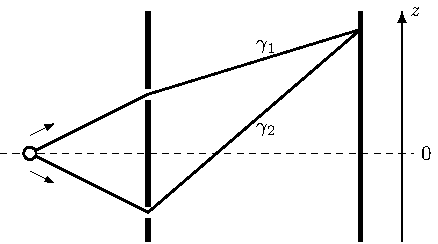
\includegraphics{fig/two_slit_free.pdf}
  \caption{自由粒子の二重スリット実験}
  \label{two_slit_free}
\end{figure}

さて,磁場がある場合の振幅を考えてみよう.このときのラグランジアンは
\begin{equation}
  L
  =
  \frac{1}{2}m\left( \dv{x}{t} \right)^2
  +
  q\bm{A}\cdot\dv{\bm{x}}{t}
  \label{lagrangian}
\end{equation}
である.ただし,今考えている状況では,電場が存在しないので
\begin{equation}
  A^{0}=\phi=0
  ,\quad
  \pdv{\bm{A}}{t}
  =
  \bm{0}
\end{equation}
という拘束がある.この下での振幅は
\begin{align}
  \ev*{x_{f}|e^{-iHT/\hbar}|x_i}
  &=
  \int_{x(0)=x_i}^{x(T)=x_f}\mathcal{D}x
  e^{iS[x]/\hbar}
  \nonumber
  \\
  &=
  \int_{x(0)=x_i}^{x(T)=x_f}\mathcal{D}x
  \exp
  \left[ \frac{i}{\hbar}S_0[x] \right]
  \exp\left[ \frac{iq}{\hbar}\int_{0}^{T}A^{i}\dv{x^i}{t}\dd t \right]
\end{align}
と書けるが,ゲージ場との相互作用項は変数変換をすれば,線積分に変換することができ,したがって経路積分の影響は受けずに外に出すことができる\footnote{
  経路積分は作用の中にある位置演算子を変数にとることになるが,積分変数になったときは経路積分の変数にはならない.正確に言うと,線積分の経路のほうが経路積分の変数になるはずだが,線積分は経路に依存しないので,経路積分については定数と見なせる.
}.結局,振幅は
\begin{equation}
  \ev*{x_{f}|e^{-iHT/\hbar}|x_i}
  =
  \exp\left[ \frac{iq}{\hbar}\int_{x_i}^{x_f}A^{i}\dd x^{i} \right]
  \int_{x(0)=x_i}^{x(T)=x_f}\mathcal{D}x
  \exp
  \left[ \frac{i}{\hbar}S_0[x] \right]  
\end{equation}
となり,経路積分は自由粒子と同様に行えばよいことになる.したがって,図\ref{two_slit_free}と同じ記法を用いれば
\begin{equation}
  I_{i}(z)
  =
  \sqrt{\frac{m}{2\pi i\hbar T}}
  \exp
  \left[ \frac{im\gamma_i}{2\hbar T} \right]
  \exp\left[ \frac{iq}{\hbar}\int_{\gamma_i}A^{i}\dd x^{i} \right]
\end{equation}
であり,
\begin{align}
  I_1(z)
  +
  I_2(z)
  &=
  \sqrt{\frac{m}{2\pi i\hbar T}}
  \exp
  \left[ \frac{im\gamma_1}{2\hbar T} \right]
  \exp\left[ \frac{iq}{\hbar}\int_{\gamma_1}A^{i}\dd x^{i} \right]
  +
  \sqrt{\frac{m}{2\pi i\hbar T}}
  \exp
  \left[ \frac{im\gamma_2}{2\hbar T} \right]
  \exp\left[ \frac{iq}{\hbar}\int_{\gamma_2}A^{i}\dd x^{i} \right]
  \nonumber
  \\
  &=
  \sqrt{\frac{m}{2\pi i\hbar T}}
  \exp
  \left[ \frac{im\gamma_1}{2\hbar T} \right]
  \exp\left[ \frac{iq}{\hbar}\int_{\gamma_1}A^{i}\dd x^{i} \right]
  \left[  
    1
    +
    \exp
    \left[  
      \frac{im\Delta\gamma}{2\hbar T}
      +\frac{iq}{\hbar}\oint A^{i}\dd x^{i}
    \right]
    \vphantom{\dfrac{\dfrac{1}{2}}{2}}
  \right]
\end{align}
となるため,強度は
\begin{equation}
  f(z)
  \sim
  \cos^2
  \left(  
    \frac{k\Delta\gamma(z)}{2}
    +
    \frac{q}{2\hbar}\oint A^{i}\dd x^{i}
  \right)
\end{equation}
である.これは,自由粒子のときの強度\eqref{intensive_free}から$\cos$の位相がズレていることを意味する.これがアハラノフ・ボーム効果である.この現象は,古典論的な直感に大きく反している.古典的には「一部の」干渉縞だけが磁場の影響を受けると考えられるからである.次の章では,この現象についての解釈を考えていこうと思う.


\section{議論}

前章では,ゲージ場の影響によって,位相が
\begin{equation}
  \oint A^{i}\dd x^{i}
  \label{phase_diff}
\end{equation}
だけ変化することを見てきた.この章ではこの効果について,考察をしていこうと思う.なお,この章では,Stack Exchangeでの質問\cite{stack1,stack2,stack3,stack4,phys_forum1}やそこで紹介されている論文\cite{Vaidman_2012,Aharonov_2015,Aharonov_2016}を参考にしている.


\subsection{ゲージ場か電磁場か}

ここで,これまでの議論を整理してみると,次のことがわかる:
\begin{enumerate}
  \item 
  量子力学の考え方(ここでは経路積分のこと)が正しいということ.
  \item 
  ラグランジアン\eqref{lagrangian}が正しいということ.
\end{enumerate}
この2つの仮定を認めてしまえば,これまでの導出を行うことができた.特に,2つ目の観点に注目してみると,ゲージ場との相互作用のほうがより本質的に見えるし,このことを根拠にしてゲージ場が実在すると結論づけることができるのではないかと思われる.

しかしながら,ストークスの定理を用いると,位相の変化は磁束密度を用いて
\begin{equation}
  \oint
  A^{i}\dd x^{i}
  =
  \int
  (\bm{\nabla}\times\bm{A})
  \cdot
  \dd\bm{S}
  =
  \int \bm{B}\cdot\dd\bm{S}
\end{equation}
と書き直すことができる.つまり,\textbf{観測可能な量はゲージ場を用いずに書くことができる}のである.この事実は,そもそも電磁場がゲージ不変であることから,これまでの議論と矛盾する結果ではない.

\vspace{10pt}
{\small
  アハラノフ・ボーム効果をゲージ場を用いずに定式化することは一応できているようである\cite{Vaidman_2012}.
}
\vspace{10pt}

以上の議論から分かることは
\begin{itemize}
  \item 
  ラグランジアンでは,ゲージ場を用いて書かないといけない
  (ゲージ場$A$を磁束密度$B$を用いて一意的に書くことはできない)
  \item 
  観測可能な量はゲージ不変で,電磁場を用いて記述するとができる
\end{itemize}
であり,この観点から言えることは「\textbf{実在をどう定義するか}によって,実在する対象を結論づけることができる」ということである.仮に,ラグランジアンやハミルトニアンに含まれるものを実在と呼ぶならゲージ場のほうが存在すると見なされるべきだし,観測可能な量のみが実在とすれば,電磁場(というよりもゲージ不変な量)のほうが存在していると言えるのである.


\subsection{局所的か}

前節の結論でも十分だが,あの結論では少しあっけないような気がするので,個人的な興味として局所性に基づいた議論にも注目してみたい.

理論の基礎的な部分が「ある1点の情報のみで記述されている」とき,その理論は局所的であるという.これは相対論を考えるときには非常に重要な観点である.例えば,2体連成振動のハミルトニアン
\begin{equation}
  H
  =
  \frac{p_1^2}{2m_1}
  +
  \frac{p_2^2}{2m_2}
  +
  \frac{1}{2}\omega^2(x_1-x_2)^2
\end{equation}
は局所的ではない.今回議論してきたラグランジアン\eqref{lagrangian}は局所的であり,その表式を見ている限りは相対性理論の思想には矛盾しない.

しかしながら,観測量の位相の変化
\begin{equation}
  \frac{q}{2\hbar}
  \oint A^{i}\dd x^i
\end{equation}
は,非局所的な量となっている.つまり,ある点$z$の強度$f(z)$を知るためには,光源からスクリーン上の1点を結ぶ閉曲線上のゲージ場の情報が全て関わってくるのである.大雑把に言えば,ソレノイド内の磁場を切ってゲージ場が0になると,その影響が一瞬で点$z$に伝わってしまうのである.アハラノフ・ボーム効果の検証は,ゲージ場の存在の有無というよりも,このような非局所的な観測量の存在を告げたといえるのかもしれない.

\vspace{10pt}
{\small
  ちなみに,波動関数の位相の変化
  \begin{equation}
    W(\gamma)
    =
    \exp\left[ 
      \frac{iq}{\hbar}
      \oint_{\gamma} A^{i}\dd x^i \right]
  \end{equation}
  を$U(1)$ゲージ理論のウィルソンループといい,ゲージ場の量子論において構成される(ゲージ不変という意味で)オブザーバブルな量である.
}

\vspace{10pt}
{\small
  いろいろと調べていたら「そもそも私たちは電磁場を観測できているのか?」「測定可能と観測可能の違いは?」といった概念的な議論が多く新鮮だった.しかし,英語でそういった文章を読むのはすごい大変だったので,もし,ここら辺の話題が書いてある日本の文献があるなら紹介していただきたい.ただし,ここらへんの分野は物理学の中でもそんなに主流ではないと思うので,そういった意味で日本語の文献がないだけかもしれない.気になった方は,参考文献に載ってあるStack Exchangeなどからあたってみると分かりやすいだろう.
}


\clearpage
\makeatletter
\renewcommand{\appendix}{\par
  \setcounter{section}{0}%
  \setcounter{subsection}{0}%
  \gdef\presectionname{\appendixname}%
  \gdef\postsectionname{}%
  \gdef\thesection{\presectionname\@Alph\c@section\postsectionname}%
  \gdef\thesubsection{\@Alph\c@section.\@arabic\c@subsection}%
  \renewcommand{\theequation}{\@Alph\c@section.\arabic{equation}}%
  \renewcommand{\thefigure}{\@Alph\c@section.\arabic{figure}}%
  \renewcommand{\thetable}{\@Alph\c@section.\arabic{table}}%
}
\makeatother
\appendix

\section{プロパゲーターの計算}
\label{prop}

ここでは,経路積分をexactに行い,\eqref{prop_free}を導出しておく.計算は\cite{Jones}の第3章に基づく.

経路積分を実行するので,よく行われるように$t=0$から$t=T$までを$N$分割して考える.この分割を行えば,作用の積分は離散化できて
\begin{equation}
  S_{0}
  =
  \frac{m}{2\varepsilon}
  \sum_{i=1}^{N}
  (x_{i}-x_{i-1})^2
\end{equation}
である.経路積分は$x_1,\cdots,x_{N-1}$の積分に変換することができて,
\begin{equation}
  \ev*{x_{f}|e^{-iH_0T/\hbar}|x_i}  
  =
  \lim_{\varepsilon\rightarrow 0}
  \left(  
    \frac{m}{2\pi i\hbar \varepsilon}
  \right)^{N/2}
  \int\dd x_1\cdots\int\dd x_{N-1}
  \exp
  \left[  
    \frac{im}{2\hbar\varepsilon}
    \sum_{i=1}^{N}
    (x_{i}-x_{i-1})^2    
  \right]
\end{equation}
となる.ここで,積分の前の定数は規格化定数であり,この離散化の方法では値が決まっている.積分を実行すれば\footnote{
  $N$についての帰納法で
  $$
    \int\dd x_1\cdots\int\dd x_{N-1}
    \exp\left[ \frac{im}{2\hbar\varepsilon}\sum_{i=1}^{N-1}(x_i-x_{i-1})^2 \right]
    =
    \frac{1}{\sqrt{N}}
    \left(  
      \frac{m}{2\pi\hbar \varepsilon}
    \right)^{-(N-1)/2}
    \exp
    \left[ \frac{im}{2\hbar\cdot N\varepsilon}(x_f-x_i)^2 \right]    
  $$
  を示せばよい(フレネル積分なので,少し注意が必要である).
}
\begin{align}
  \ev*{x_{f}|e^{-iH_0T/\hbar}|x_i}  
  &=
  \lim_{\varepsilon\rightarrow 0}
  \left(  
    \frac{m}{2\pi i\hbar N\varepsilon}
  \right)^{1/2}
  \exp
  \left[ \frac{im}{2\hbar\cdot N\varepsilon}(x_f-x_i)^2 \right]
  \nonumber
  \\
  &=
  \sqrt{\frac{m}{2\pi i\hbar T}}
  \exp
  \left[  
    \frac{im(x_f-x_i)}{2\hbar T}
  \right]
\end{align}
を得る($T=N\varepsilon$であった).


\begin{thebibliography}{99}
    \bibitem{Tonomura_ObservationAharonovBohm_1982}
    A. Tonomura et al., \textit{“Observation of Aharonov-Bohm Effect by Electron Holography,”} Phys. Rev. Lett., vol. 48, no. 21, pp. 1443–1446, May 1982, \href{https://link.aps.org/doi/10.1103/PhysRevLett.48.1443}{doi:10.1103/PhysRevLett.48.1443}.
    \bibitem{J.J.Sakurai_ModernQuantum_1985}
    J.J. Sakurai and S.F. Tuan, \textit{Modern Quantum Mechanics,} Benjamin/Cummings Pub., 1985.

    \bibitem{stack1}
    \url{https://physics.stackexchange.com/questions/99505}
    \bibitem{stack2}
    \url{https://physics.stackexchange.com/questions/56926}
    \bibitem{stack3}
    \url{https://physics.stackexchange.com/questions/86506}
    \bibitem{stack4}
    \url{https://physics.stackexchange.com/questions/132372}

    \bibitem{phys_forum1}
    \url{https://www.physicsforums.com/threads/1016214}

    \bibitem{Vaidman_2012}
    L. Vaidman, “On the role of potentials in the Aharonov-Bohm effect,” Phys. Rev. A, vol. 86, no. 4, p. 040101, Oct. 2012, doi: 10.1103/PhysRevA.86.040101, \href{http://arxiv.org/abs/1110.6169}{arXiv:1110.6169 [quant-ph]}.
    
    \bibitem{Aharonov_2015}
    Y. Aharonov, E. Cohen, and D. Rohrlich, “Comment on ‘Role of Potentials in the Aharonov-Bohm Effect,’” Phys. Rev. A, vol. 92, no. 2, p. 026101, Aug. 2015, doi: 10.1103/PhysRevA.92.026101, \href{http://arxiv.org/abs/1604.05748}{arXiv:1604.05748 [quant-ph]}.

    \bibitem{Aharonov_2016}
    Y. Aharonov, E. Cohen, and D. Rohrlich, “Nonlocality of the Aharonov-Bohm Effect,” Phys. Rev. A, vol. 93, no. 4, p. 042110, Apr. 2016, doi: 10.1103/PhysRevA.93.042110, \href{http://arxiv.org/abs/1502.05716}{arXiv:1502.05716 [quant-ph]}.
    
    \bibitem{Jones}
    E. Jones, R. Bach, H. Batelaan, \textit{"Path integrals and the double slit,"} \href{https://doi.org/10.48550/arXiv.1504.07530}{arXiv:1504.07530 [quant-ph]}.
\end{thebibliography}

\end{document}
